\section{The Structure of \jel{} System}
\label{sec:The_Components_of_the_Jeliot_3_System}

We introduce here the different components of \jel{} system. The system contains several packages and here we explain those that are most crucial in understanding the structure of \jel{}. Packages and classes related to communication between visualization engine and \djava{} are introduced in Chapter~\ref{sec:Communications_Model}.

The functional structure of the \jel{}~3 is shown in the Figure~\ref{fig:structure_of_jeliot_3}. A user interacts with the user interface and creates the source code of the program (1). The source code is sent to the Java interpreter and the intermediate code is extracted (2 and 3). The intermediate code is interpreted and the directions are given to the visualization engine (4 and 5). A user can control the animation by playing, pausing, rewinding or playing step-by-step the animation through the user interface (6). Furthermore, the user can input data, for example, an integer or a string, to the program executed by the interpreter (6, 7 and 8).

\begin{figure}[htbp]
\begin{center}
\begin{picture}(400,250)

% BOXES, OVALS and CIRCLE
%--------------------------
%User group
\put(50,30){\circle{60}}
\put(20,0){\makebox(60,60){\f{User}}}
%User interface
\put(10,90){\framebox(80,20){\f{User interface}}}
%Source code
\put(50,200){\oval(80,50)}
\put(10,175){\makebox(80,50){\shortstack{\f{Source code}\\\f{of the program}}}}
%DJava
\put(160,160){\framebox(80,80){\shortstack{\f{Interpretation}\\\f{of the program}\\\f{code done by}\\\f{\djava{}}}}}
%Intermediate code
\put(350,200){\oval(80,70)}
\put(310,165){\makebox(80,70){\shortstack{\f{Intermediate}\\\f{code of the}\\\f{program}\\\f{execution}}}}
%Visualization engine
\put(160,60){\framebox(80,50){\shortstack{\f{Visualization}\\\f{engine}}}}
%Intermediate code Interpreter
\put(310,60){\framebox(80,50){\shortstack{\f{Intermediate}\\\f{code}\\\f{Interpreter}}}}
% VECTORS
%----------------------------
% 0. (user, user interface) (user interface, user)
\put(40,47){\vector(0,1){43}}
\put(60,90){\vector(0,-1){43}}
% 1. (user interface, source code)
\put(50,110){\vector(0,1){65}}
\put(50,110){\makebox(20,65){\f{1.}}}
% 2. (source code, djava)
\put(90,200){\vector(1,0){70}}
\put(90,200){\makebox(70,20){\f{2.}}}
% 3. (djava, intemediate code)
\put(240,200){\vector(1,0){70}}
\put(240,200){\makebox(70,20){\f{3.}}}
% 4. (intemediate code, intemediate code interpreter)
\put(350,165){\vector(0,-1){55}}
\put(350,110){\makebox(20,55){\f{4.}}}
% 5. (intemediate code interpreter, visualization engine)
\put(310,100){\vector(-1,0){70}}
\put(240,100){\makebox(70,20){\f{5.}}}
% 6. (user interface, visualization engine)
\put(90,100){\vector(1,0){70}}
\put(90,100){\makebox(70,20){\f{6.}}}
% 7. (intemediate code interpreter, visualization engine)
\put(240,80){\vector(1,0){70}}
\put(240,80){\makebox(70,20){\f{7.}}}
% 8. (visualization engine, Djava)
\put(310,110){\vector(-1,1){70}}
\put(260,130){\makebox(50,50){\f{8.}}}
\end{picture}
\caption{The functional structure of Jeliot~3.}
\label{fig:structure_of_jeliot_3}
\end{center}
\end{figure}

Different packages of \jel{}~3 are introduced in this section in the same order as in the functional structure.

\subsection{Class \jel{} }
\label{sec:Jeliot_Class}

Class \jel{} in the package \p{jeliot} is the main class of the program. It combines the different components of the program together and handles the communication between different components. When the program is started the class creates all the needed components and passes them as parameters to the user interface classes. It mainly handles the communication between the user interface (\p{jeliot.gui}) and the theater/animation engine (\p{jeliot.theater}) classes. In addition to that it invokes the thread handling the interpretation of the user programs with the \p{jeliot.launcher.Launcher} class.

\subsection{User Interface}
\label{sec:User_Interface}

The user interface of Jeliot is located in the package \p{jeliot.gui}. The structure of the user interface and the actual user interface are shown in the Figures~\ref{fig:jeliot3_UI_structure} and \ref{fig:jeliot3_UI}. The main class is \p{JeliotWindow} that extends \p{JFrame}. The frame is layed out by \p{BorderLayout}. A split pane (\p{JSplitPane}) is added in the center and a panel containing the control panel (created in \p{JeliotWindow}) and the output console (\p{OutputConsole}) is added in the south (bottom) border.


\begin{figure}[htb]
\begin{center}
\begin{picture}(300,200)
%overall frame
\put(0,0){\framebox(300,200){\ }}
%Menu bar
\put(0,170){\framebox(100,30){\f{Menu bar}}}
%Code editor
\put(0,40){\framebox(100,130){\shortstack{\f{Code editor}\\\f{or}\\\f{Code viewer}}}}
%Theatre
\put(100,40){\framebox(200,160){\shortstack{\f{Animation frame (Theater)}\\\f{or}\\\f{Error viewer}}}}
%Control panel
\put(0,0){\framebox(120,40){\f{Control panel}}}
%Output Console
\put(120,0){\framebox(180,40){\f{Output Console}}}
\end{picture}
\caption{The structure of user interface in Jeliot~3.}
\label{fig:jeliot3_UI_structure}
\end{center}
\end{figure}

In the split pane the left side is used by the code editor (\p{CodeEditor}) or the code viewer (\p{CodeViewer}). The code editor is shown during editing of the program and the code viewer during the animation of the program. Both of the text components have a line numbering component (\p{LineNumbers} on their row header). The code editor consist of an editing panel that has buttons to load, save and edit the source code. The frame has also a menu bar that is constructed partially in the \p{CodeEditor} class and partially in the \p{JeliotWindow} class.

On the right hand side of the split pane a animation engine called the\-a\-ter (\p{The\-a\-ter}) is normally shown. However, if any errors occur during the compilation or run-time of the program they are shown in the \p{Error viewer} (\p{ErrorViewer}) instead of theater.

\begin{figure}[htb]
\begin{center}
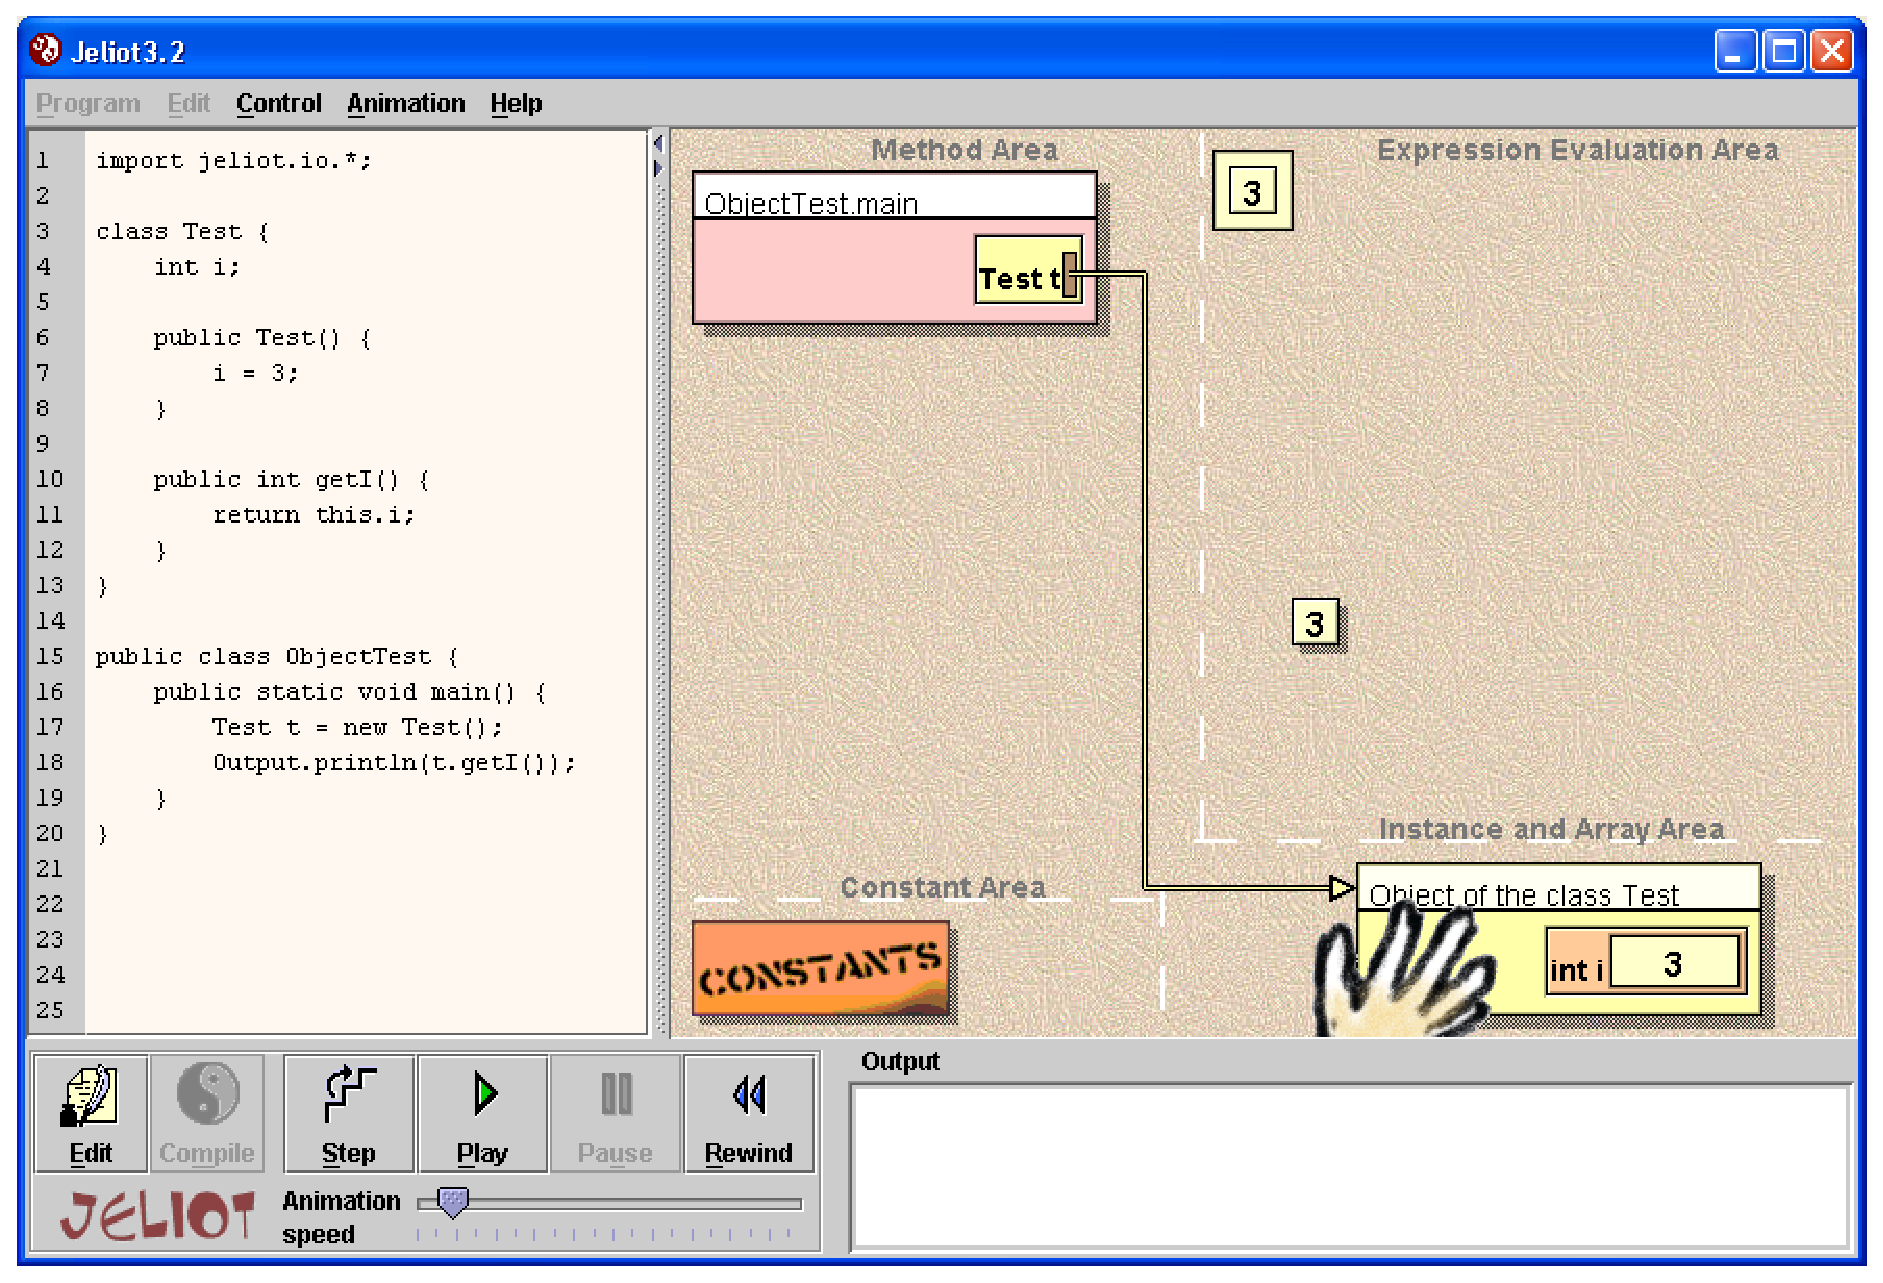
\includegraphics[width=\textwidth]{images/jeliot3.eps}
\caption{The user interface of Jeliot~3.}
\label{fig:jeliot3_UI}
\end{center}
\end{figure}

\p{JeliotWindow} combines all the components in the \p{jeliot.gui} package and creates the user interface. It also deals with most of the events happening during {run-time} and delegates the commands to the appropriate classes (e.g. \p{Jeliot} or \p{CodeEditor}). Other classes in the \p{gui} package are related to one of the components introduced in the previous paragraph.

There are also three classes that are not currently in use in \jel{}~3, namely \p{LoadJeliot}, \p{DraggableComponent} and \p{TheaterPopup}. LoadJeliot class could be used to show a splash screen in the startup of the program. DraggableComponent is an class that a DraggableComponent could extend to be dragged during the visualization. TheaterPopup class could be used to have a popup menu on the visualization frame. This popup menu could show, for example, methods of the object.

\subsection{DynamicJava}
\label{sec:DynamicJava}

\djava{} consists of 7 different packages, where only five of them actually perform the interpretation: \p{classfile}, \p{classinfo}, \p{interpreter}, \p{parser} and \p{tree}. The other two (\p{util} and \p{gui}) are used to help the debugging of \djava{} and to provide a nicer user interface to the interpreter. For example, the \p{displayVisitor}, included in the util package, provides a nice output from the syntax tree.

\begin{itemize}
\item \p{Classfile} contains all the classes for creating general purpose bytecode classes. The most important class is ClassFile which is the heart of the class creation process.

\item \p{Classinfo} contains all the classes and interfaces for using reflection on Java or interpreted classes. This package is used during the compilation of the classes.

\item \p{Interpreter} contains the classes for interpreting Java language statements. This is the most important package. It contains the most important visitors that will be explained later.

\item \p{Parser} provides the classes that compose the default parser for the language. The parser itself is represented by the class \p{Parser}. This parser has been generated by JavaCC 1.0. It creates the nodes of the tree to be traversed later by the interpreter visitors.

\item \p{Tree} provides classes and interfaces for producing an abstract syntax tree.

The created tree consists of nodes, the main data structure used in \djava{}. All nodes have common properties, the segment of source code where that node refers. Subclasses of this node are defined to address the unique properties of each different Java (e.g. staments and constructions). For example a node for any binary expression will also consist of the properties \p{LEFT\_EXRESSION} and \p{RIGHT\_EXPRESSION}.

\end{itemize}

Figure \ref{fig:Packages_visitors_and_data_flow_in_DJava} explains the main relationships between the packages, the visitors and the main data flow.

\begin{figure}[htbp]
\begin{center}
\begin{picture}(400,200)
\put(110,20){\framebox(270,130){\ }}
\put(220,20){\makebox(50,20){\f{Interpreter}}}

\put(0,50){
\put(0,15){\vector(1,0){40}}
\put(0,15){\makebox(40,20){\shortstack{\f{source}\\\f{code}}}}
\put(40,0){\framebox(50,30){\f{Parser}}}
\put(90,15){\vector(1,0){40}}
\put(90,15){\makebox(40,20){\f{tree}}}
\put(130,0){\dashbox{5}(55,30){\shortstack{\f{Name}\\\f{Visitor}}}}
\put(185,15){\vector(1,0){35}}
\put(180,15){\makebox(40,20){\f{tree}}}
\put(220,0){\dashbox{5}(55,30){\shortstack{\f{Type}\\\f{Checker}}}}
\put(275,15){\vector(1,0){35}}
\put(270,5){\makebox(40,20){\shortstack{\f{tree}\\\f{and}\\\f{class}}}}
\put(310,0){\dashbox{5}(55,30){\shortstack{\f{Evaluation}\\\f{Visitor}}}}
\put(365,15){\vector(1,0){35}}
\put(360,15){\makebox(40,20){\f{result}}}
}

\put(240,80){\vector(0,1){20}}\put(250,100){\vector(0,-1){20}}
\put(240,130){\vector(0,1){40}}\put(250,170){\vector(0,-1){40}}
\put(60,80){\vector(0,1){90}}\put(70,170){\vector(0,-1){90}}
\put(270,180){\vector(1,0){40}}\put(310,190){\vector(-1,0){40}}

\put(220,100){\dashbox{5}(55,30){\shortstack{\f{TreeClass-}\\\f{Compiler}}}}

\put(0,170){
\put(40,0){\framebox(50,30){{\f{Tree}}}}
\put(220,0){\framebox(50,30){{\f{ClassInfo}}}}
\put(310,0){\framebox(50,30){{\f{ClassFile}}}}
}

\end{picture}
\caption{Packages, visitors and data flow in \djava{}}
\label{fig:Packages_visitors_and_data_flow_in_DJava}
\end{center}
\end{figure}

As you can see, \djava{} carries the source code through three visitors: \p{NameVisitor}, \p{TypeChecker} and, finally, \p{EvaluationVisitor}. We also see how \p{EvaluationVisitor} will receive a class from \p{TypeChecker}, the reason for this behavior will be explained in the next paragraphs.

The NameVisitor is a tree visitor that resolves the ambiguity in identifiers in a syntax tree. This visitor traverses the tree trying to find out syntactical ambiguities.

The \p{TypeChecker} is a tree visitor that checks the typing rules and loads the classes, fields and methods. This \p{TypeChecker} class is not only concerned about typing rules. When visiting a class declaration, it invokes \p{TreeCompiler}, which compiles the class into Java bytecode. However, this compiling process \textit{alters the class} and the generated bytecode \textit{does not match the original source code} of the class.

The \p{EvaluationVisitor} is a tree visitor that evaluates each node of a syntax tree. This visitor is the one that performs the evaluation and execution of the program. It usually starts by invoking the main method of the compiled class. We can easily observe how it traverses the syntax tree and modifies \djava{} structures to store information and thus we can interfere with its normal interpretation to extract the information it produces while interpreting the source code.

\subsubsection{Tree package}
\label{sec:Tree_package}

The \p{Tree} package contains a class for every different Java language construct. These classes build up the syntactical tree from the source code. These classes are also implemented as a
tree. The root of this tree is the class \p{Node}. Every other class inherits it, directly or indirectly. \p{Node} only defines one property, the location of the node in the source code, both the filename and the position inside the file. \jel{} only accept single file programs, thus the filename is not needed. Most of the other classes also define properties that later are inherited by more specific classes.

The tree structure is shown in the Figures~\ref{fig:several_tree_classes}, \ref{fig:primary_expression_classes}, \ref{fig:statement_classes} and \ref{fig:un_and_bin_exp_classes}. These figures do not try to be exhaustive. Some classes have been taken away to not clutter the diagrams and because they were not needed to understand the
tree structure.

Figure~\ref{fig:several_tree_classes} shows the different nodes for declarations, initializers and types. Two main types are used by \djava{}: Array type and and primitive types (\p{int}, \p{char},\ldots). The type String is not considered as a different type as it is a class. It is Java that supports it by normal String methods.

\begin{figure}[!htb]
\begin{center}
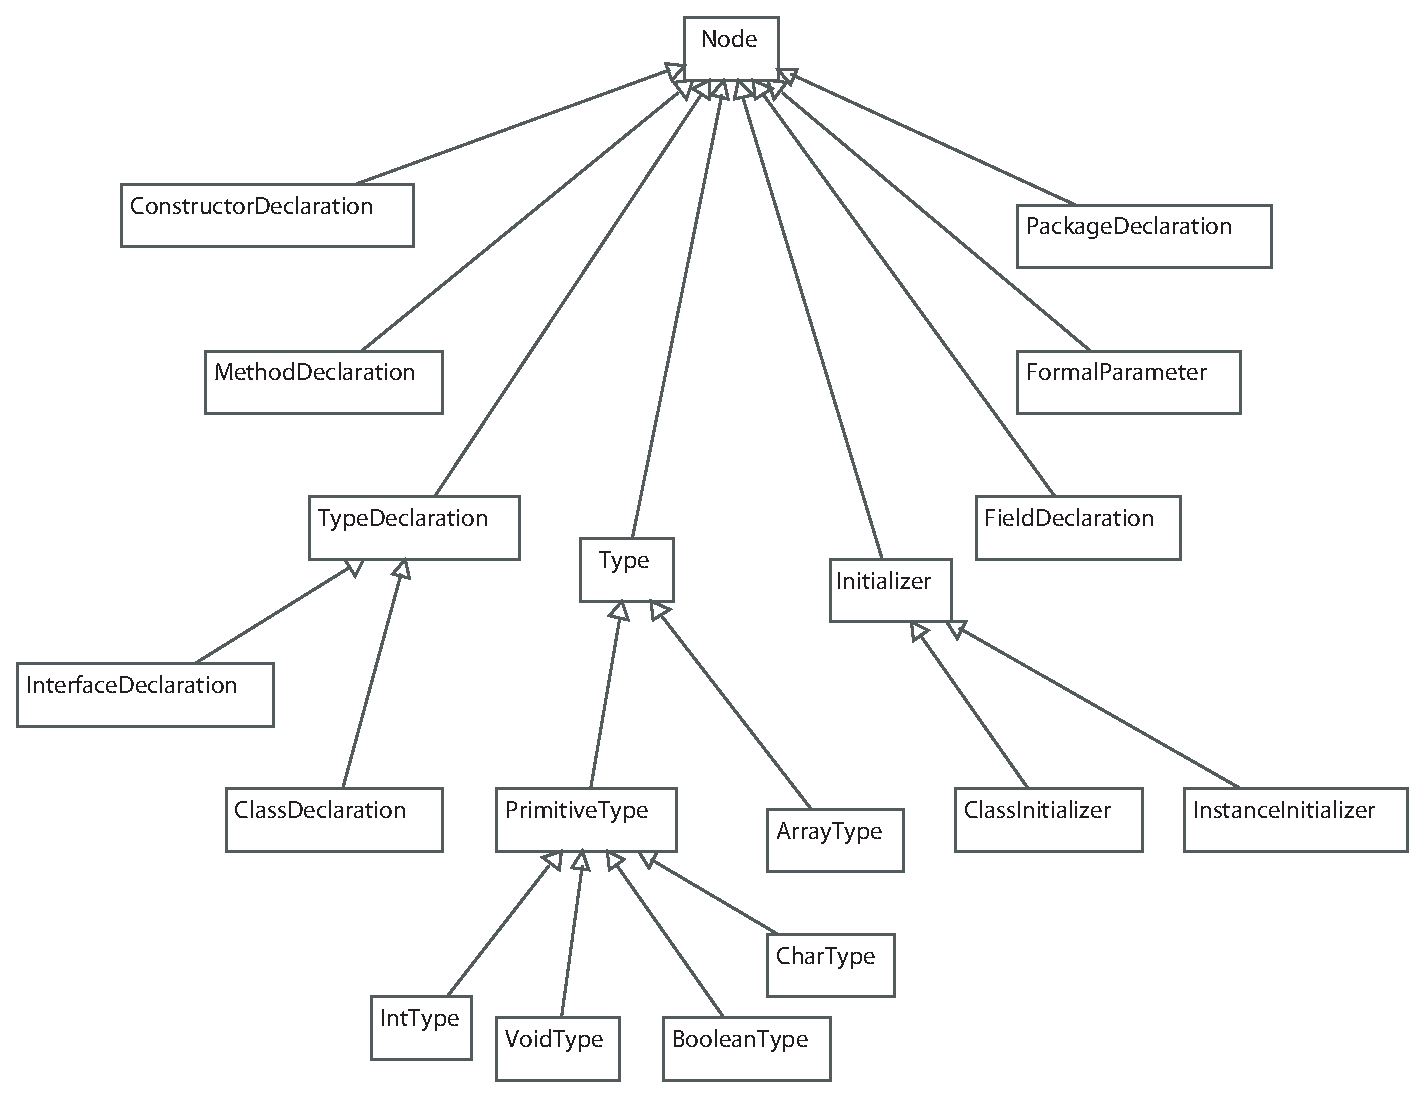
\includegraphics[width=\textwidth]{images/several.eps}
\caption{Several Tree classes. (Change the caption)}
\label{fig:several_tree_classes}
\end{center}
\end{figure}

Figure~\ref{fig:primary_expression_classes} shows the primary expressions classes. Its super class, \p{Expression}, is also super class for binary and unary expressions. All properties are defined by \p{PrimaryExpression} subclasses. Some of those also implement interfaces, even more than one. Interfaces are used by \djava{} to know when certain conditions hold. Nodes that implement \p{LeftHandSide} interface (\p{ArrayAccess}, \p{QualifiedName}, \p{FieldAccess}) are available to be the left hand side of an assignment. Those that implement \p{ExpressionContainer}
(\p{ObjectMethodCall}, \p{ReturnStatement}, \p{Constructor\-Invocation}, \p{ObjectFieldAccess},
\p{Array\-Ac\-cess}, \p{UnaryExpression}) are those that need another expression to be complete and meaningful. For example, an array access ({\tt buffer[3]} needs a qualified name ({\tt buffer}) where to look for the data, that qualified name is the expression contained in \p{ArrayAccess}. The interface \p{ExpressionStatement} is used only when \djava{} parses the source code to build the \p{ForStatement} node.

\begin{figure}[!htb]
\begin{center}
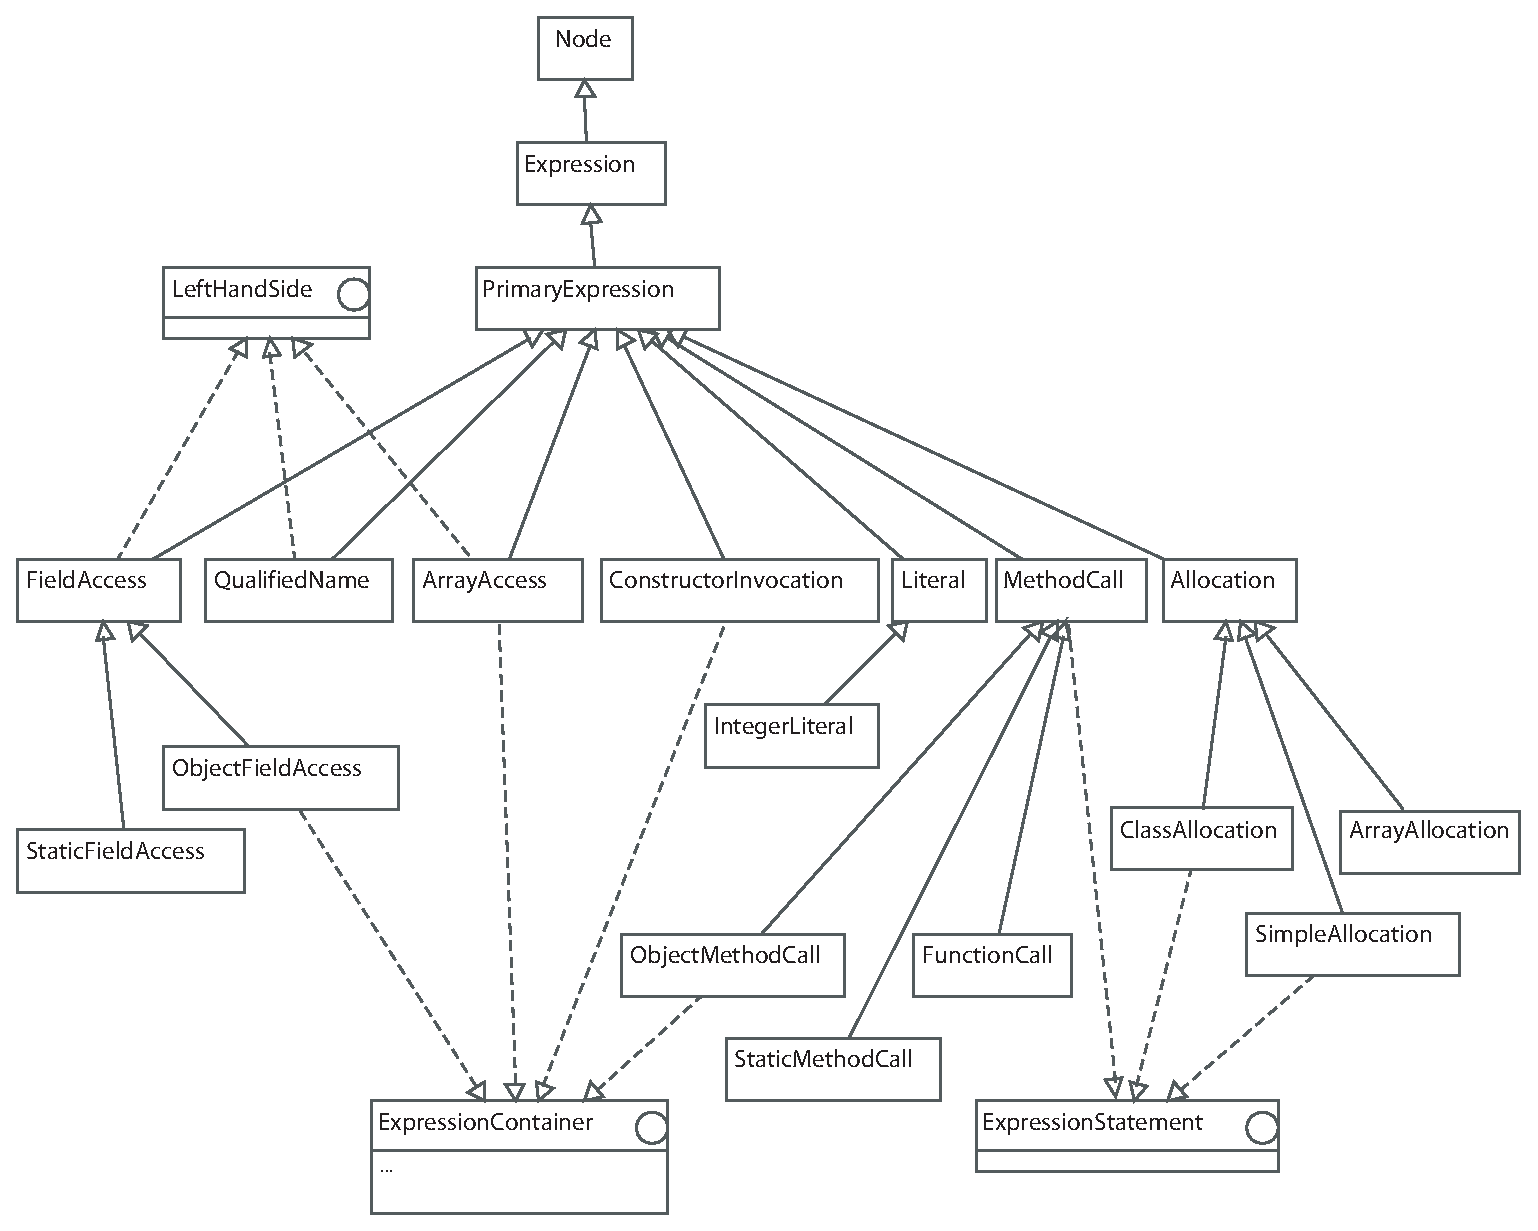
\includegraphics[width=\textwidth]{images/primaryexpressions.eps}
\caption{Primary expressions classes in \p{tree} package. (Change the caption)}
\label{fig:primary_expression_classes}
\end{center}
\end{figure}

Figure~\ref{fig:statement_classes} contains all the possible Java statements. \p{ReturnStatement} implements \p{ExpressionContainer} because it needs, that interface when it is returning an expression. \p{Do}, \p{While} and \p{For} statements implements the \p{ContinueTarget} interface in order to allow \p{ContinueStatements} inside of them.

\begin{figure}[!htb]
\begin{center}
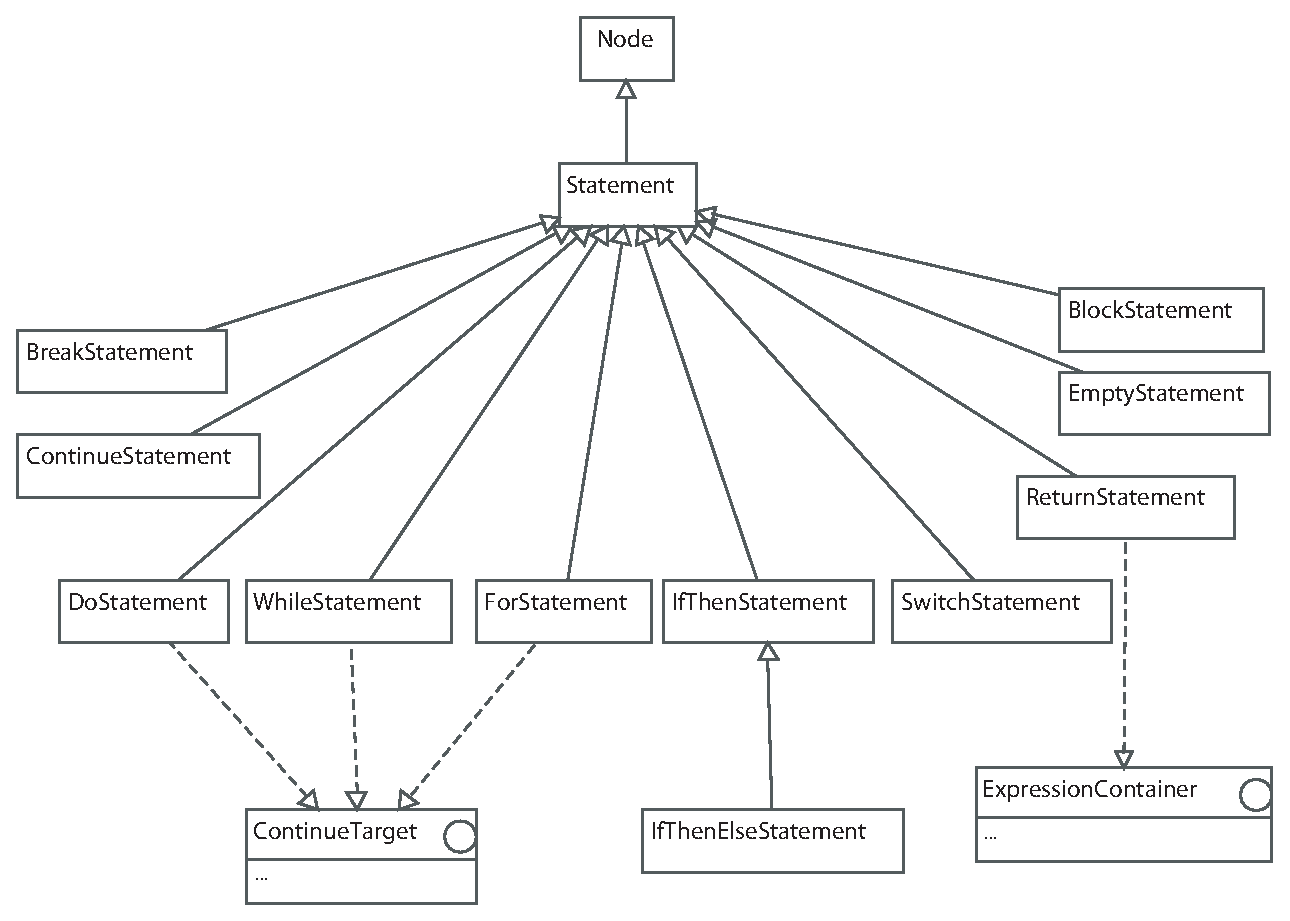
\includegraphics[width=\textwidth]{images/statements.eps}
\caption{Statement classes in \p{tree} package. (Change the caption)}
\label{fig:statement_classes}
\end{center}
\end{figure}

Figure~\ref{fig:un_and_bin_exp_classes} illustrates unary and binary expressions. It shows one as an example of each their subclasses. So \p{AndExpression} also refers to \p{OrExpression} and so on.

\begin{figure}[!htb]
\begin{center}
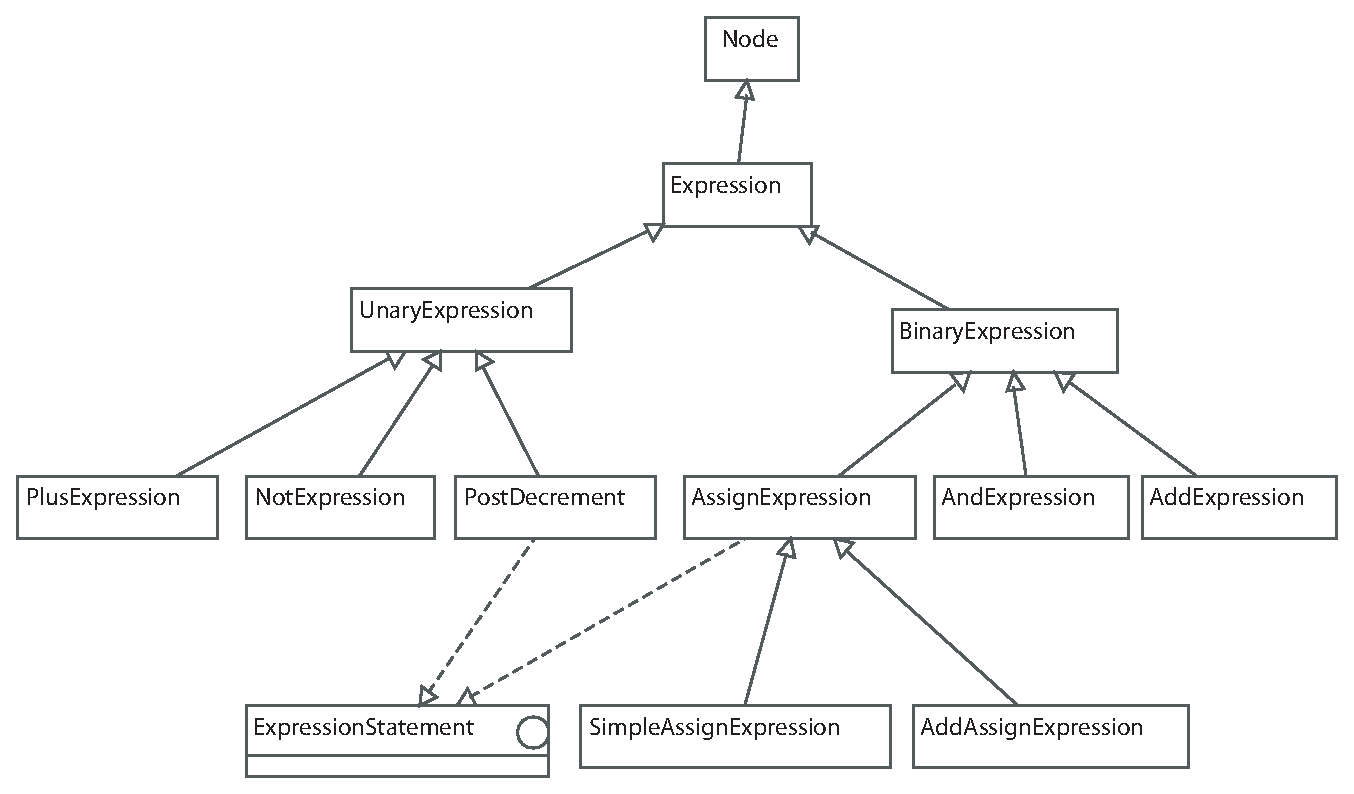
\includegraphics[width=\textwidth]{images/unary-bin-exps.eps}
\caption{Unary and binary expression classes in \p{tree} package. (Change the caption)}
\label{fig:un_and_bin_exp_classes}
\end{center}
\end{figure}

\subsection{Intermediate Code Interpreter}
\label{sec:Intermediate_Code_Interpreter}

The package \p{jeliot.mcode} includes the classes used by the intermediate code interpreter. The class \p{Interpreter} contains the intermediate code interpreter and the other classes that  help the work with intermediate code generation, interpretation and on the other aspects of the program execution.

The intermediate code is generated by the modified version of \djava{}. The code is then written into a pipe that can be read by the interpreter. As the code is completely machine written we know the form of the code and can interpret it easily. The intermediate code is introduced in the section~\ref{sec:Intermediate_Code}. The code is read line by line and it is tokenized with the agreed token in the class \p{Code} that contains all the necessary constants for intermediate code generation. Then the first token tells what kind of statement is coming and how it should be processed. The rest of the statement is processed accordingly and a part of the animation is shown if necessary.

There are several important data structures in the \p{Interpreter} class:
\begin{description}

\item[\p{commands}] variable is a reference to a stack (\p{Stack}) that contains information about each command read. Command in this context tells, for instance, whether a operand of a binary operation is the left or right side of the operation.

\item[\p{exprs}] variable is a reference to a stack (\p{Stack}) containing the information about each expression read. The information consists of each expression's type (e.g. addition or subtraction operation), reference and location in the code. It is used to identify which operands (i.e. values or variables) belong to which operation.

\item[\p{values}] variable is a reference to a hash table (\p{Hashtable}) that contains the values of literals, variables and operations encountered during the execution. Each of the values is stored in a form of \p{Value} object containing also \p{ValueActor} object of that value if it is already available. The expression reference is used as a key for the hash table. These values are then used when an expression evaluation is animated.

\item[\p{variables}] variable is a reference to a hash table (\p{Hashtable}) that contains the visited variables as instances of the \p{Variable} class. Each instance also contains \p{VariableActor} instance as an attribute. The expression references are used as the keys in the hash table. These values are used for expressions when a variable reference is needed and the value of the variable is not enough, for example, in pre- and postincrements.

\item[\p{instances}] variable is a reference to a hash table (\p{Hashtable}) that contains the instances (an object of \p{Instance} class or its subclasses) that are currently instantiated in the program. The keys of the hash tables are the hash values of the instances, which means that the instances used in the program must generate unique hash values.

\item[\p{currentMethodInvocation}] variable is a refernce to an array which has a component type \p{Object}. Array \p{currentMethodInvocation} keeps track of all the information about the method invocation. The cells of the array contain the following information: method name (\p{String}), Class/Object expression (\p{String}), Parameter values (Array of \p{String}s), Parameter types (Array of \p{String}s), Parameter names (Array of \p{String}s), Highlight information for invocation (\p{Highlight}), Highlight information for declaration (\p{Highlight}), Parameter expression references (\p{Integer}), Object reference if method is constructor or object method (\p{Integer}).

\item[\p{methodInvocation}] variable is a reference to a stack (\p{Stack}) that keeps the information of the method invocations both the current and the previous but still active invocations. Each time a method invocation is closed the stack is popped and the previous invocation record is set as the new \p{currentMethodInvocation}.

\item[\p{postIncsDecs}] variable is a reference to a hash table (\p{Hashtable}) that keeps the information about all the post increments or decrements that should be performed. This information is collected when a intermediate code command for post increment or decrement is read. The expression reference is used as the key in the hash table. During every expression involving variables, it is tested if the post increment or decrement should be animated after the variable value is used in the visualization.

\item[\p{currentClass}] variable is a reference to an instance of \p{ClassInfo} class that contains the information about the constructors, methods and fields that each class has. 

\item[\p{classes}] variable is a reference to an instance of \p{Hashtable} that contains the \p{ClassInfo} instances of all the classes that are created.

\item[\p{objectCreation}] variable is a reference to an instance of \p{Stack} that contains the hash code of the current object allocation during the constructor call.

\item[\p{returned, returnValue, returnActor, returnExpressionCounter}] are variables for handling the return value of a method.

\end{description}

Class \p{MCodeUtilities} is used by the interpreter to help type identification and translating the intermediate code into the commands used in the visualization engine. For example, visualization engine uses same numbers for binary and unary expression and the difference is made with the method call, whereas in intermediate code binary and unary expressions have different numbers as their codes. \p{MCodeUtilities} also handles some issues related to user input and communication between \djava{} and the intermediate code interpreter.

\subsection{Language Constructs}
\label{sec:Language_package}

The classes of \p{jeliot.lang} package represent Java language constructs. They are mainly used to store and transfer the information about these language construct for the creation and storing of the corresponding \p{Actor}s (see section~\ref{sec:Actors}). The Figure~\ref{fig:language_constructs_and_actors} shows the class structure of the language construct classes and the corresponding \p{Actor}s that are used as attributes of the language constructs.

\begin{figure}[!htb]
\begin{center}
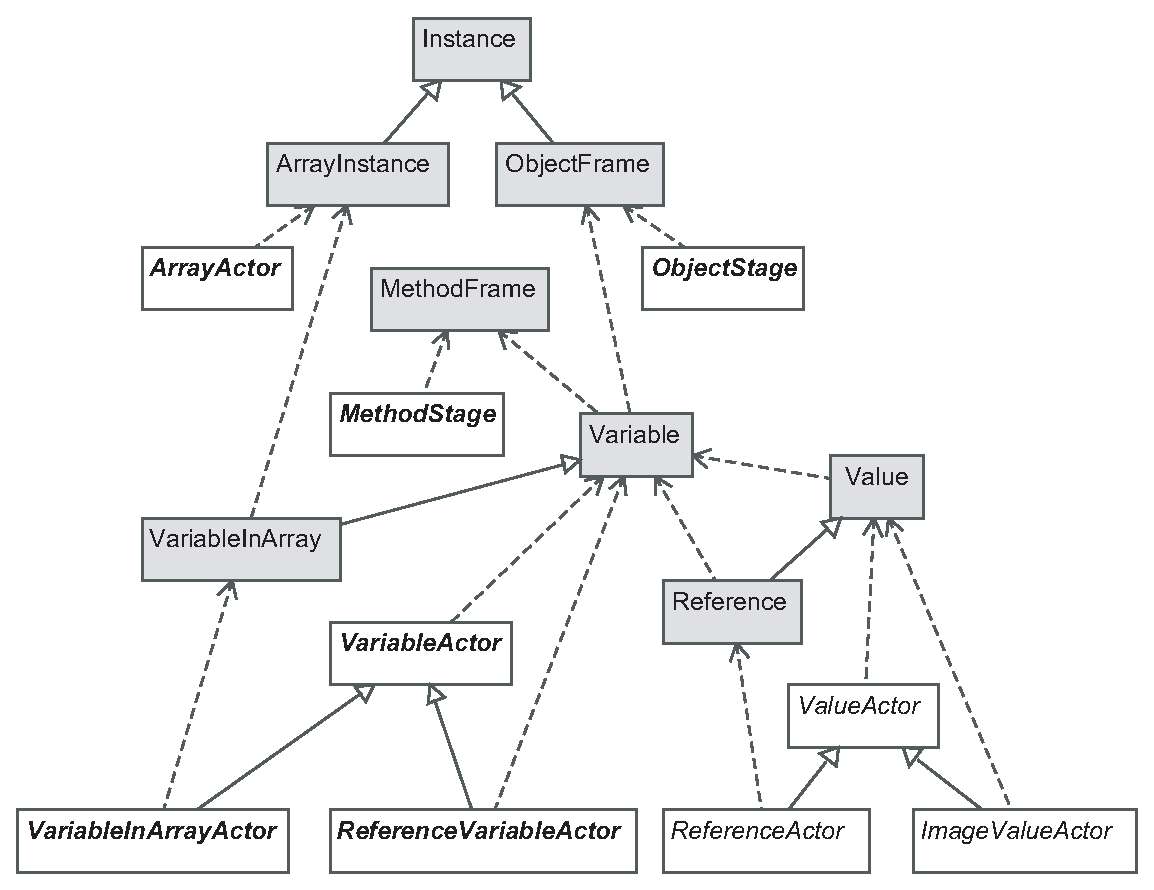
\includegraphics[width=\textwidth]{images/language_constructs_and_actors.eps}
\caption{The class hierarchy of the language constructs (gray boxes and solid lines) and the \p{Actor}s (white boxes and solid lines) and their usage relations to each other (dashed lines). \p{Actor}s (white boxes) implementing actor container are written in bold and italics and the other \p{Actor}s on just italics (see section~\ref{sec:Actors}).}
\label{fig:language_constructs_and_actors}
\end{center}
\end{figure}

\p{Instance} class is the base class for all the instances (e.g. \p{ArrayInstance} and \p{ObjectFrame}).
The instance of the \p{ArrayInstance} class represents an array of n-dimensions. 
The instance of the \p{ObjectFrame} represents an object of a class that is created at runtime. 

The instance of the \p{ClassInfo} class contains the information about a single Java class. It contains all the fields, methods and constructors of the class. 

The instance of the \p{MethodFrame} class represents a method under execution. A method frame is created runtime each time a method is called.

The instance of the \p{Variable} class is an instance of a variable --- a field or a local variable. A new variable is created runtime every time a local variable is declared. The instance of the \p{VariableInArray} is an instance of an array variable. A new array variables are created at runtime every time a new array is created.

The instance of the \p{Value} class represents any primitive type of value and values of String type and is the base class for reference values. The instance of the \p{Reference} is a value of a reference type meaning that all the references to the instances are objects of this class. 

\subsection{Visualization Engine}
\label{sec:Visualization_Engine}

The package \p{jeliot.theater} contains classes that are used to form the animation of the program. We will here introduce the most important classes in the package and explain the meaning of these classes. For rest of the classes see their source codes.

\subsubsection{Director class}

\p{Director} has methods for different kinds of operations during the animation of the program (e.g. binary expression, unary expression, object creation and method call). These methods are called by the intermediate code interpreter (\p{MCodeInterpreter}). In each of the methods are given parameters that the method needs for the operation.

Normally, the method first creates actors through \p{ActorFactory} or uses existing actors. \p{Animation}s are created through \p{Actor}s' methods (e.g. \p{appear} or \p{fly}). Created animations are given to the \p{AnimationEngine} to be run. Actors can be also added to other \p{ActorContainer}s (e.g. \p{Theater}, \p{VariableActor} or \p{MethodStage}).

\subsubsection{Actor classes}
\label{sec:Actors}

There is a large number of different \p{Actor} classes as can be seen from Figure~\ref{fig:class_hierarchy_of_Actor_class_small}. 

\begin{figure}[!htb]
\begin{center}
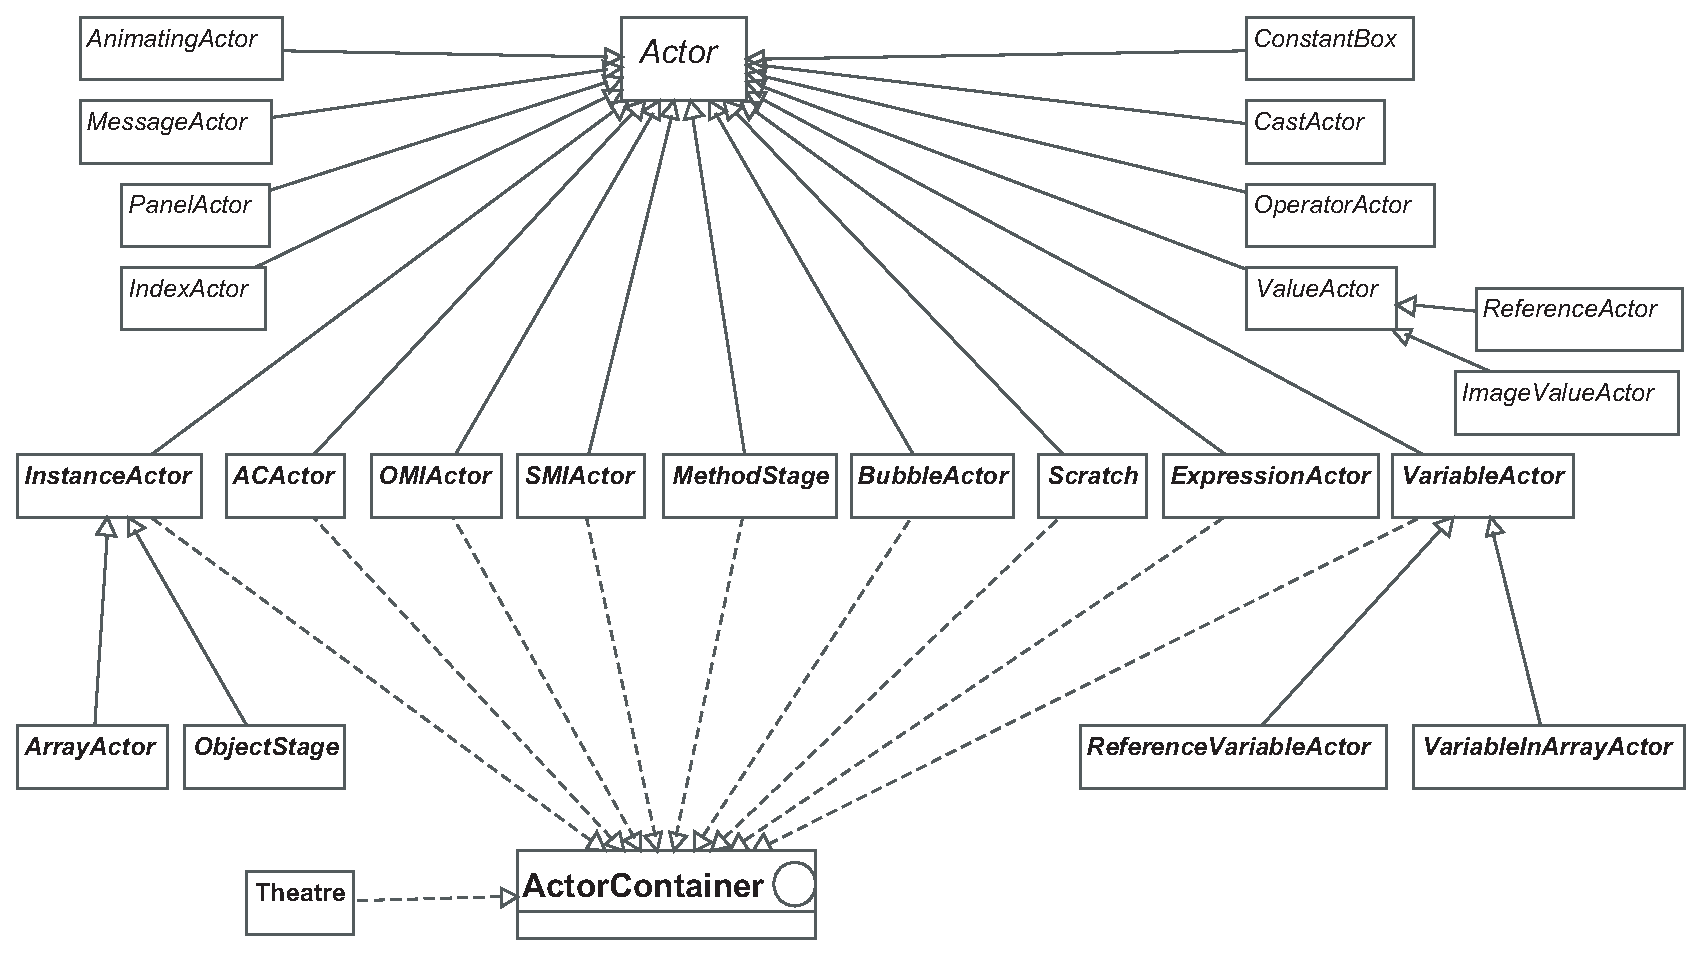
\includegraphics[width=\textwidth]{images/jeliot_actor_class_small.eps}
\caption{The class hierarchy of \p{Actor} class and \p{ActorContainer} interface.}
\label{fig:class_hierarchy_of_Actor_class_small}
\end{center}
\end{figure}

\p{Actor} class is the base class for all the actors. The \p{Actor} class should not be used directly but indirectly with it's subclasses. 

\p{ValueActor} is an actor that represents graphically the language construct \p{Value}. The \p{Value}'s type is represented by the colors of the \p{ValueActor} and the \p{Value}'s value is printed out as the String representation of the value. \p{ImageValueActor} is an actor that is used when a value actor should be an image. At the moment this only happens when the value of a variable is unknown visualized as ``???''. \p{ReferenceActor} shows the reference to some \p{InstanceActor} (e.g. \p{ArrayActor} or \p{ObjectStage}). They can be assigned to the \p{ReferenceVariableActor} instances or any other instance that is derived from the \p{ReferenceVariableActor}.

An instance of the \p{OperatorActor} class represents a operator in  the expressions. It can be a binary or unary operator and it is shown in the \p{ExpressionActor} with the operands. 

\p{Scratch} controls the expression evaluation area. It allocates the space for each \p{ExpressionEvaluationActor} and possibly for other \p{Actor}s that are there temporarily. \p{ExpressionActor} represents a single line of a scratch the evaluation area. It can contain any number of different \p{Actor}s (e.g. \p{ValueActor}, \p{ReferenceActor}, \p{OperatorActor}, \p{SMIActor}, \p{OMIActor} or \p{BubbleActor}) inside that it renders.

\p{VariableActor} represent graphically the language construct \p{Variable} for primitive data types and Strings. \p{ReferenceVariableActor} represents graphically the variables of the reference type. It can bind \p{ReferenceActor} instances and render them. \p{VariableInArrayActor} represent graphically the language construct \p{VariableInArray} for primitive data types and Strings. 

\p{SMIActor} represents graphically the static method invocation. The actor shows the  method name and the parameters in a similar way as Java syntax just replaces the variable references with their actual values. \p{OMIActor} represents graphically the object method invocation. The actor shows the object reference, the method name and the parameters in a similar way as Java syntax just replaces the variable references with their actual values.

\p{MethodStage} is the graphical representation of the \p{MethodFrame}. It contains the local \p{VariableActor}s and handles the scope changes.

\p{InstanceActor} is a base class for all the instances: \p{ArrayActors} and \p{Object\-Stage}. An instance of this class should not be instantiated. \p{Object\-Stage} is the graphical representation of the \p{ObjectFrame}. It contains the field of the object as \p{VariableActor}s. \p{ArrayActor} represents the array instance and contains \p{Var\-i\-a\-ble\-In\-Array\-Actor}s for every index of the array. \p{IndexActor} shows the line between the array access' indexing expression result value and the array's actual index. 

\p{BubbleActor} is used to move the return value from the \p{MethodStage} to the \p{ExpressionActor} on the \p{Scratch} (evaluation area).

\p{CastActor} handles the animation of the casting of the primitive values.

\p{ConstantBox} instance represents a place where all the literal constants appear during the animation.

\p{AnimatingActor} is a actor that may be used to show frame based animation. The output animation is currently uses this actor.

The \p{LinesAndText} actor draws the dashed lines and titles to separate explicitly the theater (animation frame) into four areas: constant area, method area, object and array area and expression evaluation area.

\p{MessageActor} shows all the textual messages to the user. 

\p{PanelActor} represents the curtains of the theater and produces the opening and closing animations of the curtains.

\subsubsection{ActorContainer interface}

\p{ActoContainer} interface is implemented by classes that are going to contain \p{Actor}s as their fields and take care of their painting. This means that those classes having actors as their fields but not taking care of the painting of the actors are not implementing this class. The implementing classes are shown in Figure~\ref{fig:class_hierarchy_of_Actor_class_small}. The different containing relationships are illustrated in Figure~\ref{fig:actors_and_actorcontainers}.

\begin{figure}[!htb]
\begin{center}
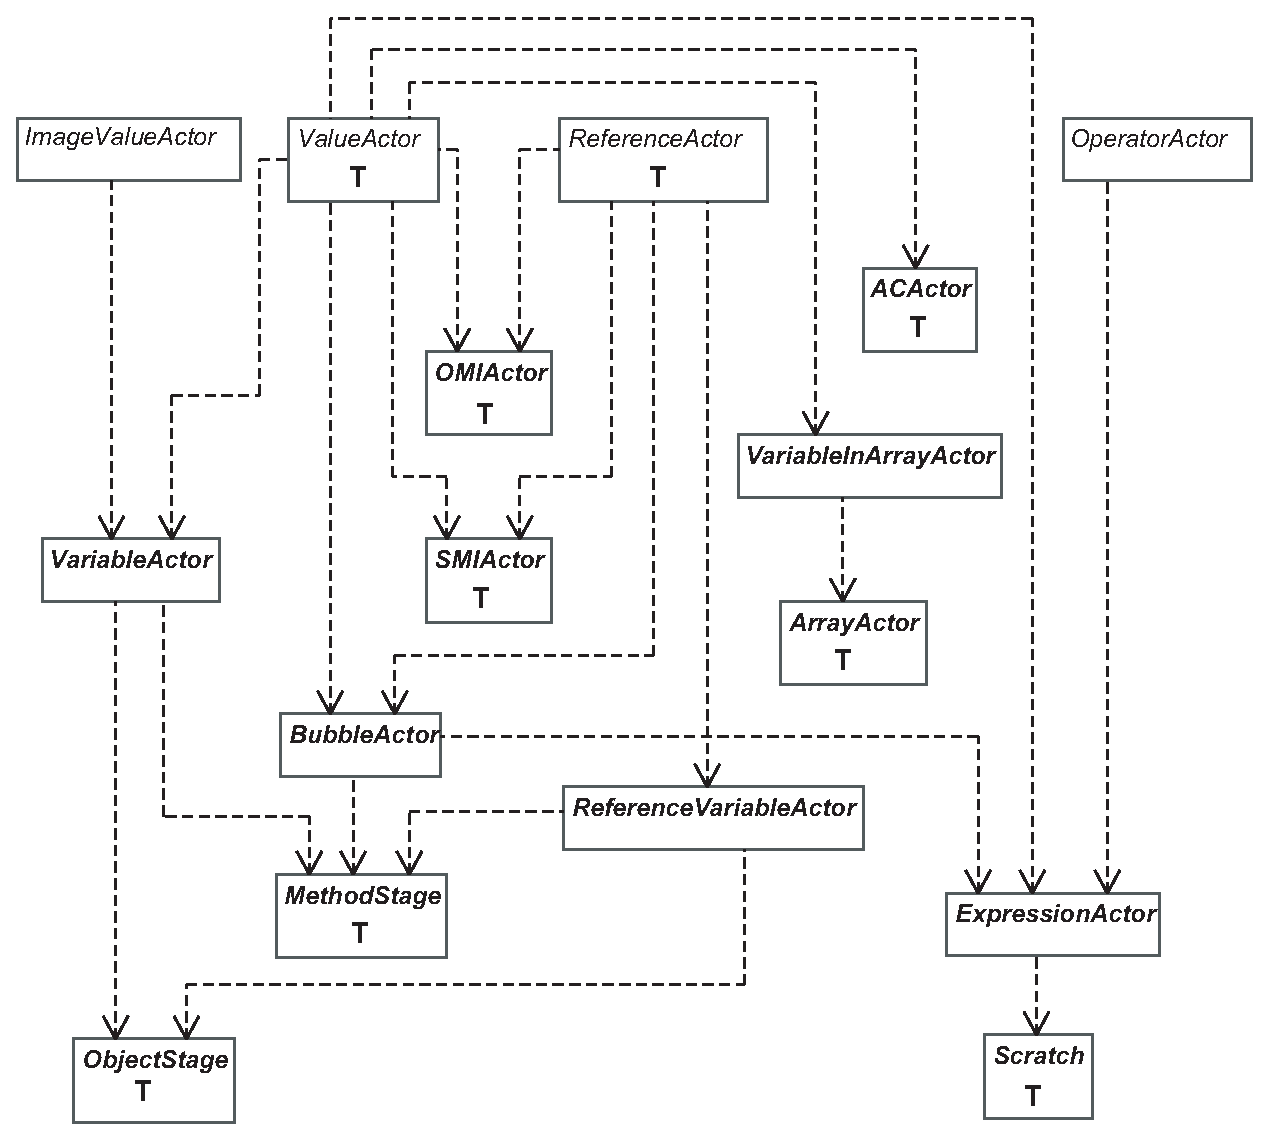
\includegraphics[width=10cm]{images/actorcontainers_and_actors.eps}
\caption{The inclusion relations between \p{Actor}s and \p{Actor}s implementing \p{ActorContainer} interface.}
\label{fig:actors_and_actorcontainers}
\end{center}
\end{figure}

\subsubsection{ActorFactory class}

This class handles the centralized creation of all the \p{Actor}s. This enables the centralized appearance handling for fonts, color and other appearance parameters. If the appearance parameters of the actors are going to be changed this class should be consulted first before any modifications to the actual \p{Actor} classes are made.

\subsubsection{Animation class}

\p{Animation} class represents one atomic animation in \p{Jeliot}. Animation means here any event that includes movement of actors or that is otherwise dependent of time. Examples of animation include moving an actor from one place to another or flashing the colors of an actor as it is introduced to the theatre.

The animation is played by an instance of \p{AnimationEngine} class. The animation engine takes care of scheduling the animation. Animation class is the abstract superclass of various specialized animation classes. These subclasses must implement the \p{animate} method in which they make their changes to actors. The animation engine calls this method at even time intervals. If the animation has to do something in prior to starting the animation, especially if it has to set any parameters that depend on the duration of the animation or it has to add any actors to the theater, it may do this in its \p{init()} method. When the animation finishes, the engine calls its \p{finish} method.

See from Figure~\ref{fig:jeliot3_animation_engine} how the \p{Animation} class relates to the animation formation.

\subsubsection{AnimationEngine class}

\p{AnimationEngine} schedules the animations represented by instances of \p{An\-i\-ma\-tion} class. The engine is given an animation or an array of animations, and it plays those animations. The speed and quality of the animation can be controlled by setting its volume (speed) and FPS (Frames Per Second) values. An engine's volume is the amount of action it gives to the animation objects each second. The higher the volume, the faster the animations will play.

An animation engine may be assigned a \p{ThreadController} instance. In this case, the engine checks with the controller after every step of animation calling its \p{checkPoint} method.

See from Figure~\ref{fig:jeliot3_animation_engine} how the \p{AnimationEngine} relates to the animation formation.

\begin{figure}[!htb]
\begin{center}
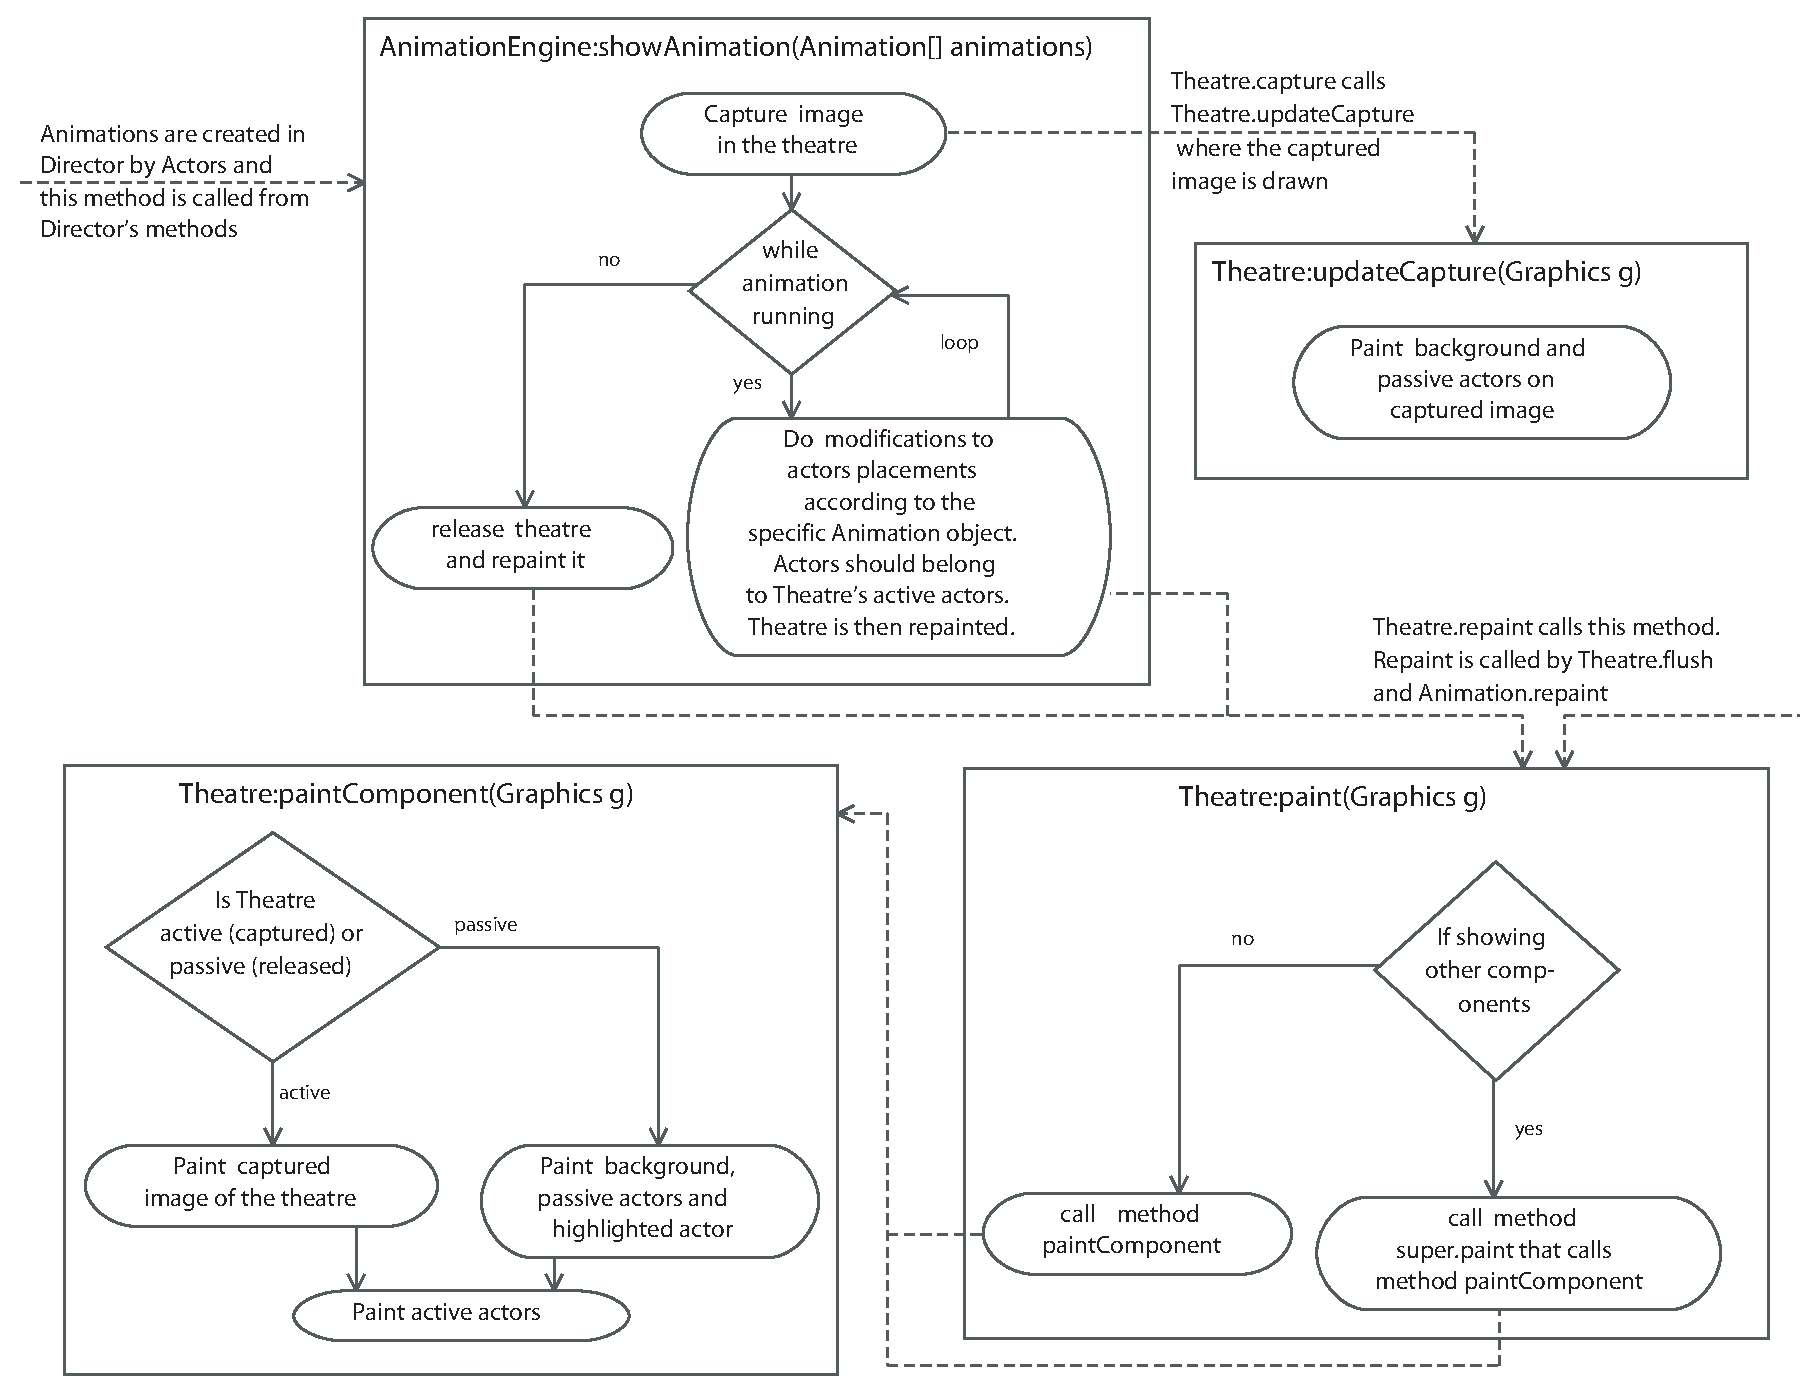
\includegraphics[width=\textwidth]{images/jeliot_animation_engine3.eps}
\caption{The structure of the animation engine in \jel{}.}
\label{fig:jeliot3_animation_engine}
\end{center}
\end{figure}

\subsubsection{Theater class}

The \p{jeliot.theater} package contains a class \p{Theater} that extends \p{JComponent} class so that it can be entered inside the split pane in the user interface. It is the canvas for the animation and all the actors are drawn on it. The different actors of the theater are shown on the theater in different areas that are shown in  Figure~\ref{fig:jeliot3_theatre_structure}. Furthermore, the \p{TheaterManager} allocates the places for the
different actors on these areas.

\begin{figure}[htbp]
\begin{center}
\begin{picture}(250,200)
%Overall frame
\put(0,0){\framebox(250,200){{\f{\bf{Theater}}}}}
%Method frame area
\put(10,100){\dashbox{5}(80,90){\shortstack{\f{Method}\\\f{Stage}\\\f{Area}}}}
%Constant box
\put(10,10){\dashbox{5}(60,30){\shortstack{\f{Constant}\\\f{Box}}}}
%Instance Area
\put(80,10){\dashbox{5}(160,80){\shortstack{\f{Instance}\\\f{Area}}}}
%Expression Evaluation Area
\put(100,110){\dashbox{5}(140,80){\shortstack{\f{Expression}\\\f{Evaluation}\\\f{Area}\\\f{(Scratch)}}}}
\end{picture}
\caption{The structure of the animation frame (theater) in Jeliot~3.}
\label{fig:jeliot3_theatre_structure}
\end{center}
\end{figure}

\p{Theater} instance is a special case of an \p{ActorContainer} because actually \p{The\-a\-ter} is not a subclass of the \p{Actor} class but still is implements \p{ActorContainer} interface. The \p{Theater} contains two different kinds of \p{Actor}s. The other actors are active (stored into \p{Vector} \p{actAct}) and the other actors are passive (stored into \p{Vector} \p{pasAct}). The active actors are the one that are drawn every time again when the new round of the animation is run. The passive actors are only stored in the background image in the beginning of the animation to optimize the drawing during the animation. See Figure~\ref{fig:theatre_and_actorcontainers} for those actors that are inserted as active actors during the animations.

\begin{figure}[!htb]
\begin{center}
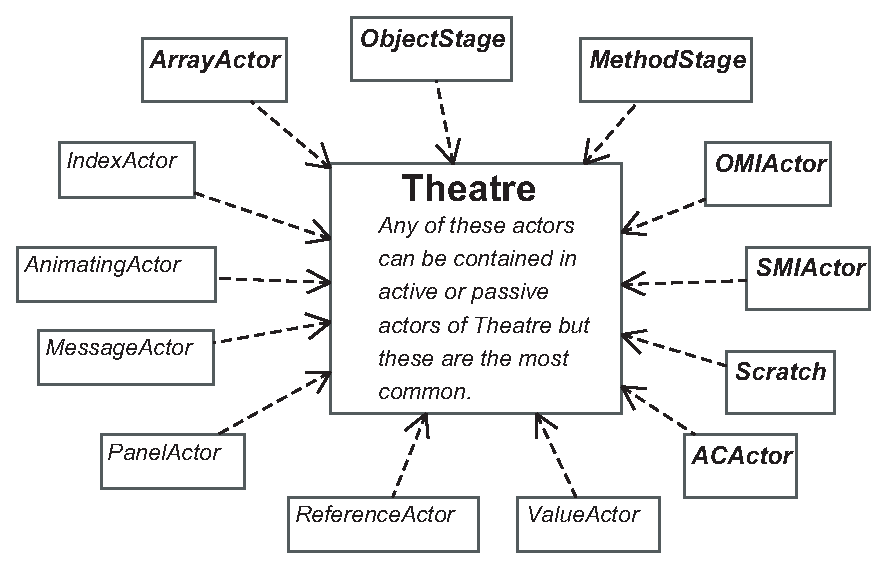
\includegraphics[width=10cm]{images/theatre_and_actors.eps}
\caption{The \p{Actor}s that are commonly included in the passive (\p{pasAct}) and active (\p{actAct}) \p{Actor}s.}
\label{fig:theatre_and_actorcontainers}
\end{center}
\end{figure}

See from Figure~\ref{fig:jeliot3_animation_engine} how the \p{Theater} relates to the animation formation.

\subsubsection{TheaterManager class}

\p{TheaterManager} allocates the space for all \p{InstanceActor}s, \p{MethodStage}s, \p{Scratch}\-es and constants (\p{ConstantBox}), and also listens the \p{Theater} component for resizes so the the allocation of the space is valid after resizing of the \p{Theater} component.